%%%% Better Poster latex template example v1.0 (2019/04/04)
%%%% GNU General Public License v3.0
%%%% Rafael Bailo
%%%% https://github.com/rafaelbailo/betterposter-latex-template
%%%% 
%%%% Original design from Mike Morrison
%%%% https://twitter.com/mikemorrison

\documentclass[a3paper,fleqn]{betterposter}

%%%% Uncomment the following commands to customise the format

%% Setting the width of columns
% Left column
\setlength{\leftbarwidth}{0.3\paperwidth}
% Right column
\setlength{\rightbarwidth}{0.27\paperwidth}

%% Setting the column margins
% Horizontal margin
%\setlength{\columnmarginvertical}{0.05\paperheight}
% Vertical margin
%\setlength{\columnmarginhorizontal}{0.05\paperheight}
% Horizontal margin for the main column
%\setlength{\maincolumnmarginvertical}{0.15\paperheight}
% Vertical margin for the main column
%\setlength{\maincolumnmarginhorizontal}{0.15\paperheight}

%% Changing font sizes
% Text font
% \renewcommand{\fontsizestandard}{\fontsize{28}{66} \selectfont}
% Main column font
\renewcommand{\fontsizemain}{\fontsize{110}{50} \selectfont}
% Title font
\renewcommand{\fontsizetitle}{\fontsize{60}{35} \selectfont}
% Author font
\renewcommand{\fontsizeauthor}{\fontsize{40}{35} \selectfont}
% Section font
%\renewcommand{\fontsizesection}{\fontsize{28}{35} \selectfont}

%% Changing font sizes for a specific text segment
% Place the text inside brackets:
% {\fontsize{28}{35} \selectfont Your text goes here}

%% Changing colours
% Background of side columns
%\renewcommand{\columnbackgroundcolor}{black}
% Font of side columns
%\renewcommand{\columnfontcolor}{gray}
% Background of main column
%\renewcommand{\maincolumnbackgroundcolor}{empirical}
%\renewcommand{\maincolumnbackgroundcolor}{theory}
%\renewcommand{\maincolumnbackgroundcolor}{methods}
%\renewcommand{\maincolumnbackgroundcolor}{intervention}
% Font of main column
%\renewcommand{\maincolumnfontcolor}{gray}

\begin{document}	
\betterposter{
%%%%%%%% MAIN COLUMN

\maincolumn{
%%%% Main space
``\textbf{Cancer patient\\treatment outcomes} can be improved by\\\textbf{identifying sources of\\uncertainty} when\\quantifying the\\biological effect of\\radiation.''\\

}{
%%%% Bottom space

%% QR code
\begin{center}
    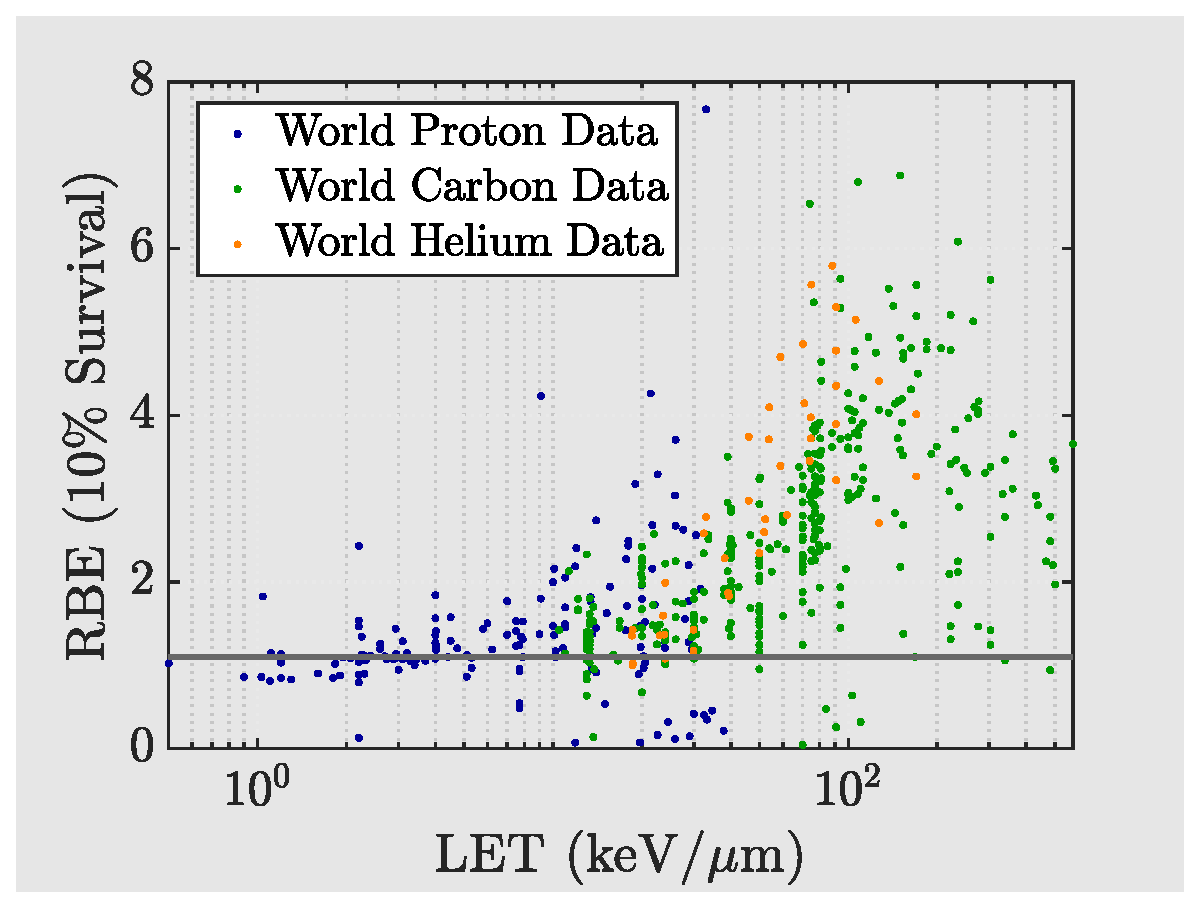
\includegraphics[width=0.8\textwidth]{RBE_worlddata.eps}\\
    \caption{\fontsize{66}{}{Figure 1}}
\end{center}
\qrcode{}{}{}

% Smartphone icon
% Author: Freepik
% Retrieved from: https://www.flaticon.com/free-icon/smartphone_65680

%% Compact QR code (comment the previous command and uncomment this one to switch)
%\compactqrcode{img/qrcode}{
%\textbf{Take a picture} to
%\\download the full paper
%}

}

}{
%%%%%%%% LEFT COLUMN

\title{Reducing Uncertainty in Proton Therapy Dose-Response}
\author{Melissa Anne McIntyre}
\section{Introduction}

\begin{itemize}
\item Key objective in radiation therapy is to optimise dose-response in the patient - we want to \textbf{maximise the biological effect on the tumour} whilst \textbf{minimising impact on organs at risk}.
\item Proton Therapy optimises this effect through the \textbf{Bragg Peak} (high dose region indicated in red below).
\begin{center}
    % Picture of ducklings
    % Author: Magda Ehlers, https://www.pexels.com/@magda-ehlers-pexels
    % Retrieved from: https://www.pexels.com/photo/selective-focus-photo-of-flock-of-ducklings-perching-on-gray-concrete-pavement-1300355/
    \includegraphics[width=0.9\textwidth]{patientPBT.png}
\end{center}
\item Our understanding of the \textbf{underlying mechanisms that describe how the tumour responds} to ionising radiation can be improved.
\end{itemize}

\section{The Problems}
\begin{itemize}
    \item \textbf{Relative Biological Effectiveness (RBE)} quantifies the \textbf{doses required for photon and proton radiation to achieve the same biological effect}
    \begin{eqnarray*}
        RBE = \frac{Dose_{\text{ Photon}}}{Dose_{\text{ Proton}}}\quad .
    \end{eqnarray*}
    \item In treatment planning a \textbf{constant proton RBE of 1.1 is assumed} despite clear correlation with beam energy and linear energy transfer (LET) (Fig.1)
    \item The \textbf{RBE uncertainty increases} with LET (Fig.1)
\end{itemize}
\section{Methods}
\begin{itemize}
    \item We will simulate cell response data and identify the parameters that have the biggest impact on RBE uncertainty.
    \item Then we will test using a variable and uncertainty reduced RBE on real patient treatment plans.
    \item We except that \textbf{accounting for uncertainty} in the biological response of tissues to radiation will \textbf{improve treatment outcomes for cancer patients}.
\end{itemize}

\vfill

}{
%%%%%%%% RIGHT COLUMN
\vfill
\textbf{The underlying mechanisms of cell response to ionising radiation~:}
\vfill
Relative Dose delivered as a function of depth. The red region representing the maximum relative dose delivered is lined up with the tumour~:

\begin{center}
    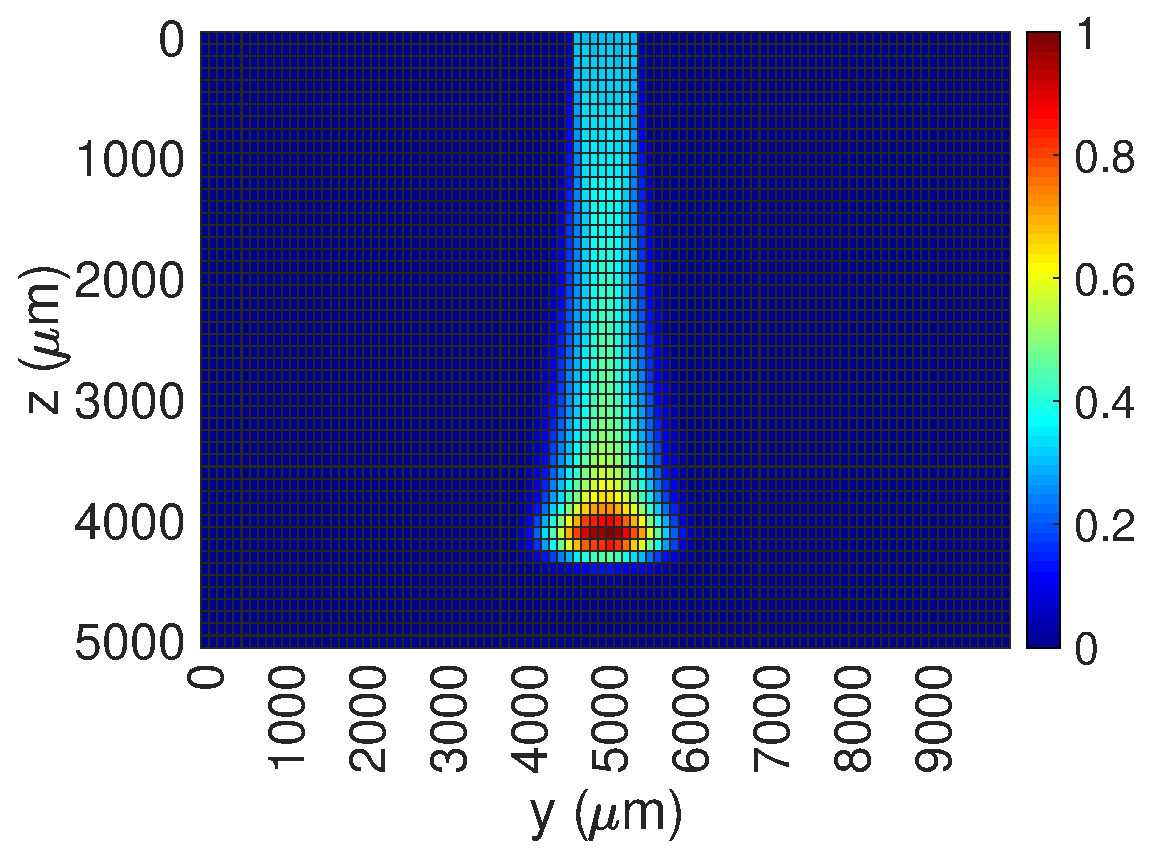
\includegraphics[width=\textwidth]{doseheatmap_depth.eps}
\end{center}

A single proton track propagating through water - each colour represents a different particle or chemical species~:
\begin{center}
% Picture of ducklings
% Author: Magda Ehlers, https://www.pexels.com/@magda-ehlers-pexels
% Retrieved from: https://www.pexels.com/photo/selective-focus-photo-of-flock-of-ducklings-perching-on-gray-concrete-pavement-1300355/
\includegraphics[scale=1.3]{chem_100ps.eps}
\end{center}
\begin{itemize}
    \item The ionisation density of the track structure determines how severely the DNA inside the cells within the tumour are damaged.
\end{itemize}

\begin{center}
    % Picture of ducklings
    % Author: Magda Ehlers, https://www.pexels.com/@magda-ehlers-pexels
    % Retrieved from: https://www.pexels.com/photo/selective-focus-photo-of-flock-of-ducklings-perching-on-gray-concrete-pavement-1300355/
    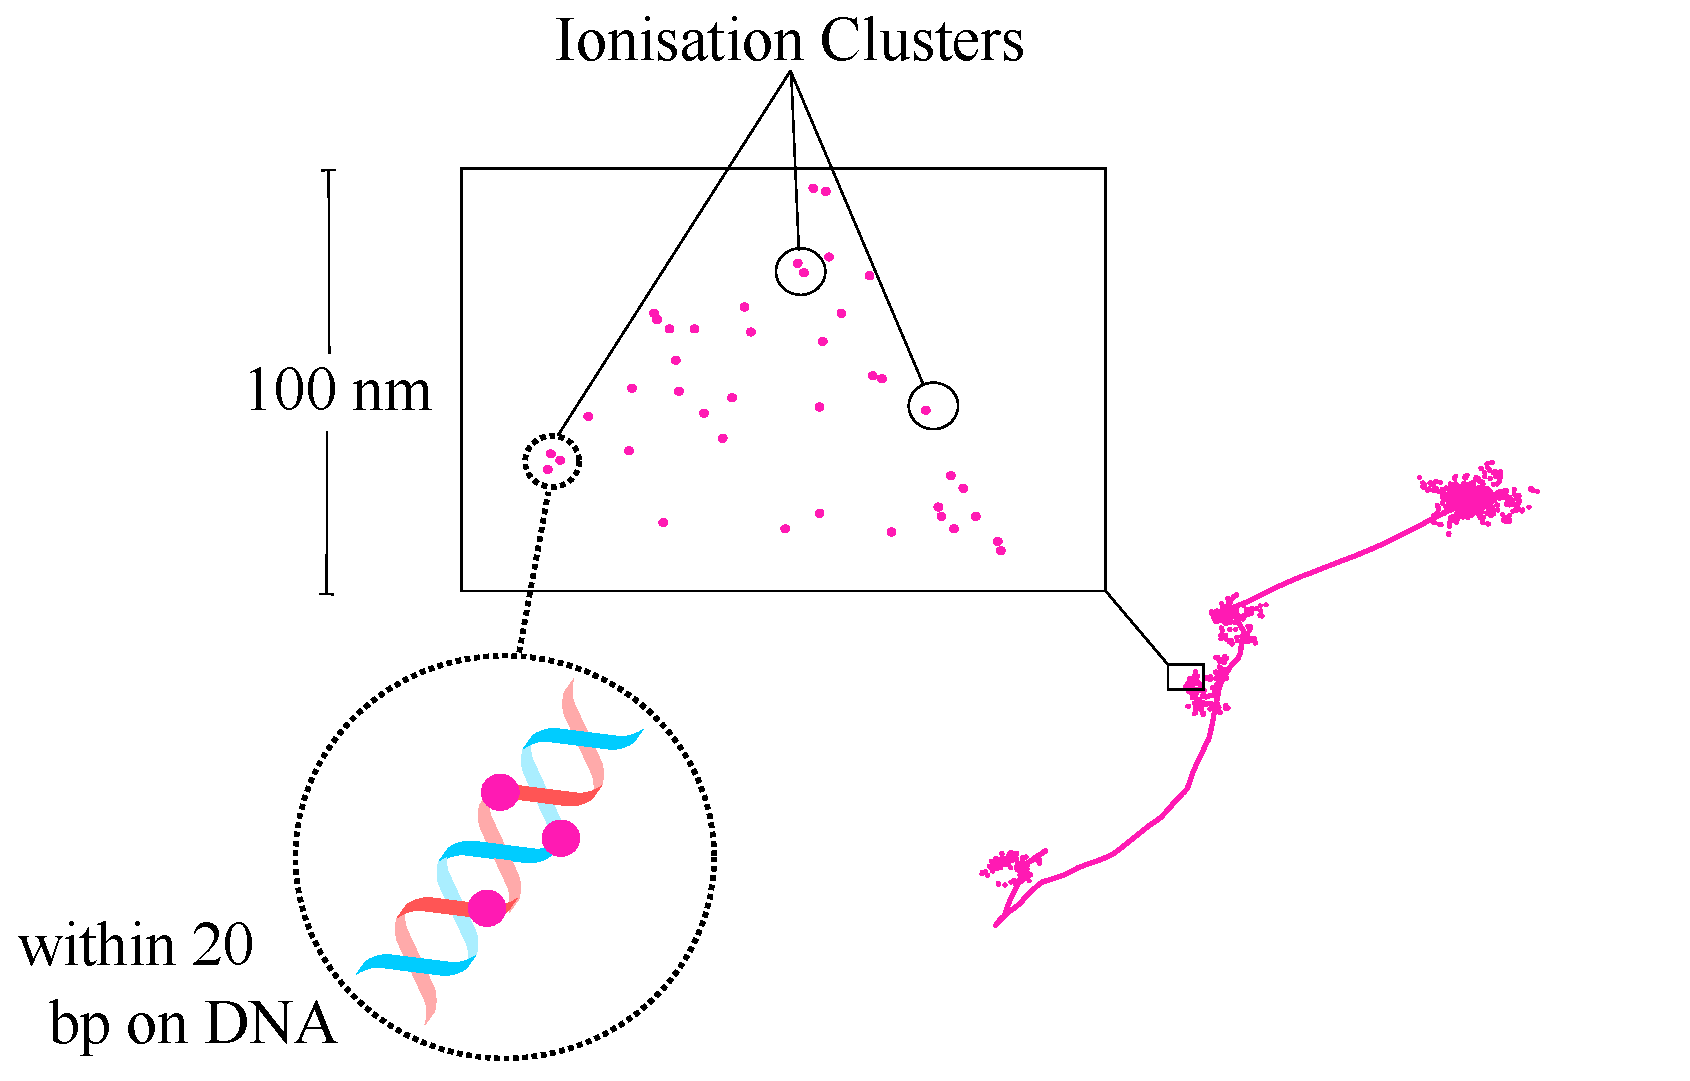
\includegraphics[scale=0.8]{ionisationcluster_zoomedout.eps}
\end{center}

\begin{itemize}
    \item When the particle tracks damage the DNA severely enough, the cancer cells will deactivate causing the tumour to shrink.
\end{itemize}
\vfill
}
\end{document}
